\documentclass{article}

\usepackage[preprint]{neurips_2025}

\usepackage[utf8]{inputenc}
\usepackage[T1]{fontenc}
\usepackage{hyperref}
\usepackage{url}
\usepackage{booktabs}
\usepackage{amsfonts}
\usepackage{amsmath}
\usepackage{nicefrac}
\usepackage{microtype}
\usepackage{xcolor}
\usepackage{graphicx}

\title{Assignment 2: EGNN Ablation Archaeology}

\author{%
  Leonardo Mattos Martins \\
  Boston University \\
  \texttt{leom@bu.edu}
}

\begin{document}

\maketitle

\begin{abstract}
Equivariant Graph Neural Networks naturally enforce physical symmetries directly in their architecture. This approach proves highly effective for molecular and particle dynamics. This report presents a systematic ablation study of an EGNN predicting long-horizon simulations of charged particles under Coulomb interactions. I evaluate several components including distance inputs in messages coordinate tanh bounding initialization velocities residual connections and general coordinate equivariance itself. The results establish that unconstrained coordinate updates and loss of spatial distance information severely degrade prediction accuracy. Removing the tanh bounding on coordinate updates leads to catastrophically exploding trajectories yielding the highest Mean Squared Error (26.08). Conversely breaking equivariance destroys geometric generalization leading to high equivariance error despite moderate training stability. Other components like residual connections supply necessary but comparatively minor optimization benefits. I additionally introduce an attention-weighted modification to edge passing that significantly improves upon the baseline error by enhancing expressive capacity for learning Coulomb interactions.
\end{abstract}

\section{Introduction}

Equivariant Graph Neural Networks (EGNNs) learn on physical systems while preserving continuous group symmetries. These specifically include the E(n) transformations of translation rotation and reflection in coordinate space. Rather than relying on computationally heavy data augmentation where a network must learn invariances implicitly through brute force EGNNs bake strict geometric symmetries directly into their computation graphs. 

When observing physical phenomena such as many-body interacting charged particles influenced by Coulomb forces the fundamental forces remain independent of the absolute origin of the system. They also rotate consistently with any spatial rotation vector. Consequently EGNNs represent graphs using both node specific properties like mass and charge alongside the Cartesian coordinates and momenta of the nodes as spatial embeddings. Edges pass scalar messages representing interactions but the spatial coordinate update explicitly treats relative distance vectors as directions to perturb position and velocity. 

This study aims to discover the relative importance of specific EGNN mechanisms through systematic ablation archaeology. I expect to verify that core invariant inputs like relative distance and exactly equivariant coordinate transformations are essential for low prediction error in dynamics tasks. Conversely I suspect other features such as residual structures and specific nonlinear squashing functions like tanh clamping primarily assist stable optimization rather than act as fundamental requirements for achieving equivariance. 

\section{Ablation Study}

\subsection{Experimental Design}

I trained six variant networks to observe changes in final Validation Mean Squared Error (MSE) and overall Rotational Equivariance error over a 100-epoch training session on simulated charged particle dynamics. The Equivariance Error test randomly generates orthogonal rotation matrices R and tests if the model output commutes with the transformation: $f(Rx, Rv) \approx R \cdot f(x, v)$.

The tested network variations include the following:
\begin{itemize}
    \item \textbf{Full EGNN}: The complete baseline equivariant network.
    \item \textbf{\texttt{egnn\_no\_equivariance.py}}: I break explicit rotation and translation symmetry by concatenating the node absolute position vector into the generated message scalars ($m_{ij}$).
    \item \textbf{\texttt{egnn\_no\_velocity.py}}: Velocity vectors initialize as zeros instead of leveraging input momentum. This demands the network approximate acceleration and final momentum using solely positions and charges.
    \item \textbf{\texttt{egnn\_no\_distance.py}}: Geometrical scalar messages bypass node distance metrics ($||x_i - x_j||^2$) and lean exclusively upon discrete charge embeddings between interacting neighbors.
    \item \textbf{\texttt{egnn\_no\_tanh.py}}: I remove bounded velocity shift predictions inside message propagation.
    \item \textbf{\texttt{egnn\_no\_residual.py}}: I prevent features from sequentially accumulating via skip connections.
    \item \textbf{\texttt{egnn\_improved.py}}: I generate logits scaled by softmax along local edges to introduce dynamic attention weights instead of homogeneous message aggregation.
\end{itemize}

\subsection{Results}

\begin{table}[h]
  \centering
  \begin{tabular}{lcc}
    \toprule
    \textbf{Model} & \textbf{Validation MSE} $\downarrow$ & \textbf{Equivariance Error} $\downarrow$ \\
    \midrule
    \texttt{egnn\_improved.py} & 0.0092 & $8.45 \times 10^{-7}$ \\
    Full EGNN Baseline & 0.0766 & $8.30 \times 10^{-7}$ \\
    \texttt{egnn\_no\_residual.py} & 0.0781 & $7.28 \times 10^{-7}$ \\
    \texttt{egnn\_no\_velocity.py} & 0.0863 & $7.66 \times 10^{-7}$ \\
    \texttt{egnn\_no\_equivariance.py} & 0.0903 & $1.17 \times 10^{-2}$ \\
    \texttt{egnn\_no\_distance.py} & 0.1068 & $7.51 \times 10^{-7}$ \\
    \texttt{egnn\_no\_tanh.py} & 26.0826 & $1.09 \times 10^{-4}$ \\
    \bottomrule
  \end{tabular}
  \caption{Validation MSE and calculated rotational Equivariance Error measured up to floating-point precision on the testing environment. The Improved Attention model achieves the best performance while the No Tanh model diverges.}
  \label{tab:ablation-results}
\end{table}

\vspace{-0.2cm}

\begin{figure}[h]
  \centering
  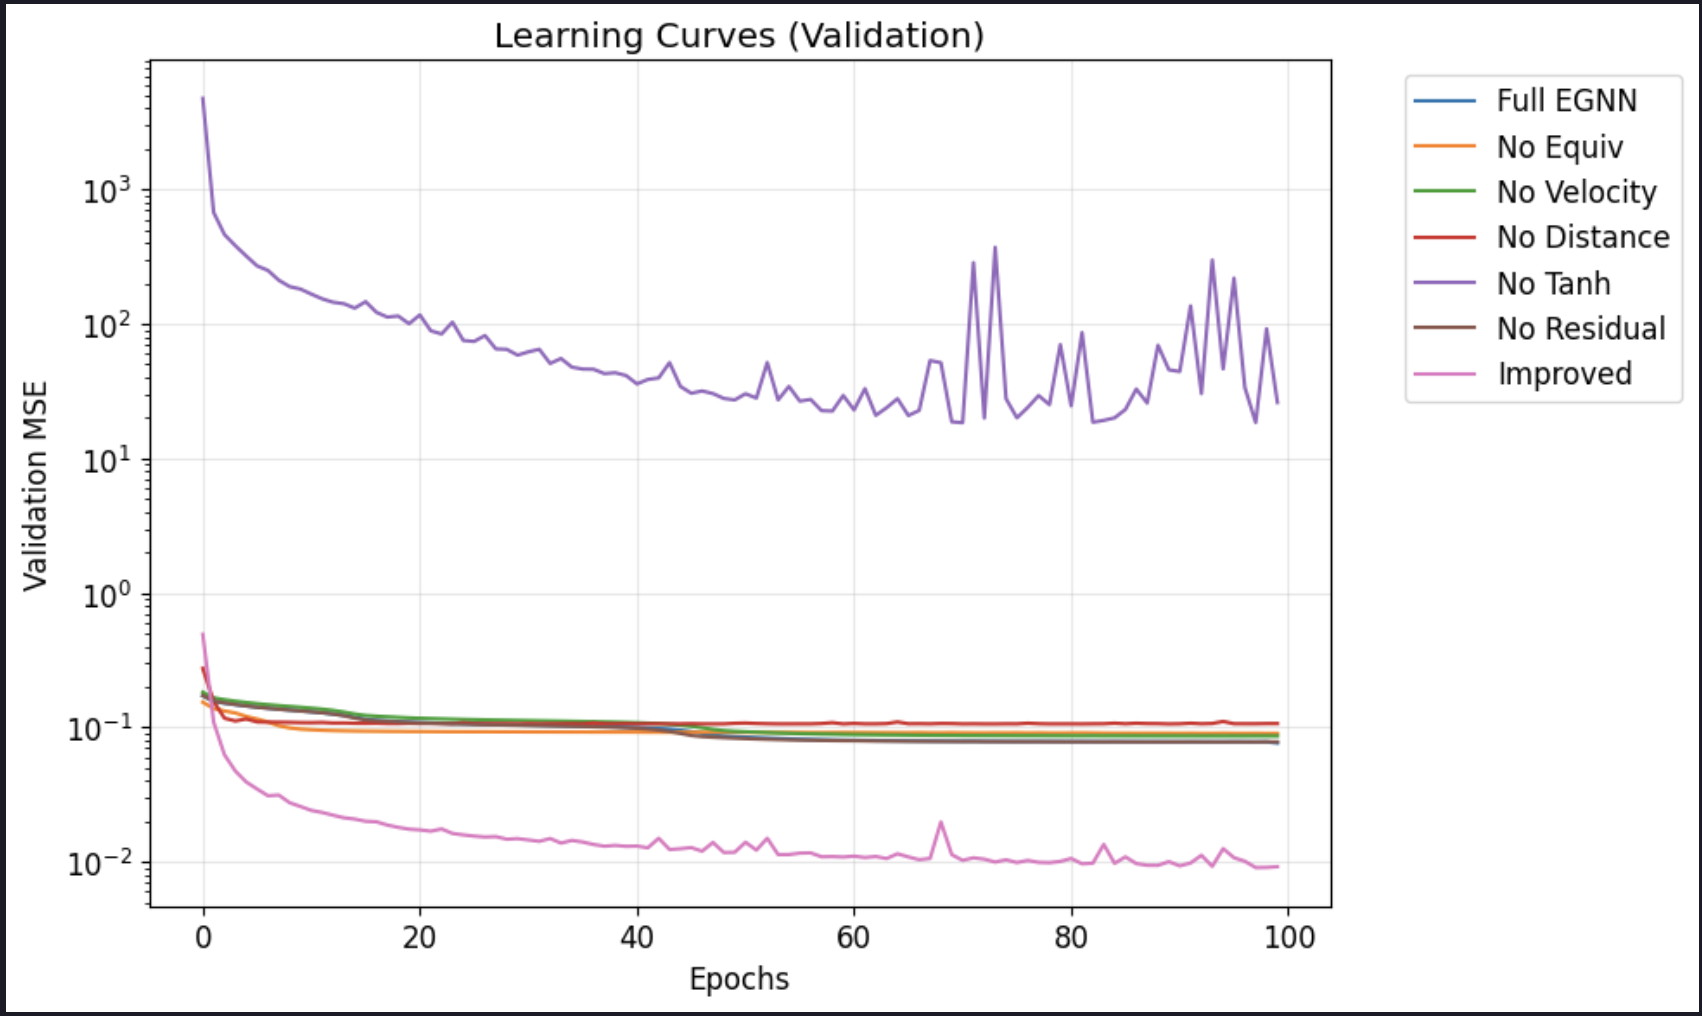
\includegraphics[width=0.45\textwidth]{learning_curve.png}
  \vspace{-0.2cm}
  \caption{Validation learning curves across 100 epochs demonstrating relative stability and convergence floors.}
\end{figure}

\begin{figure}[h]
  \centering
  \begin{minipage}{0.49\textwidth}
    \centering
    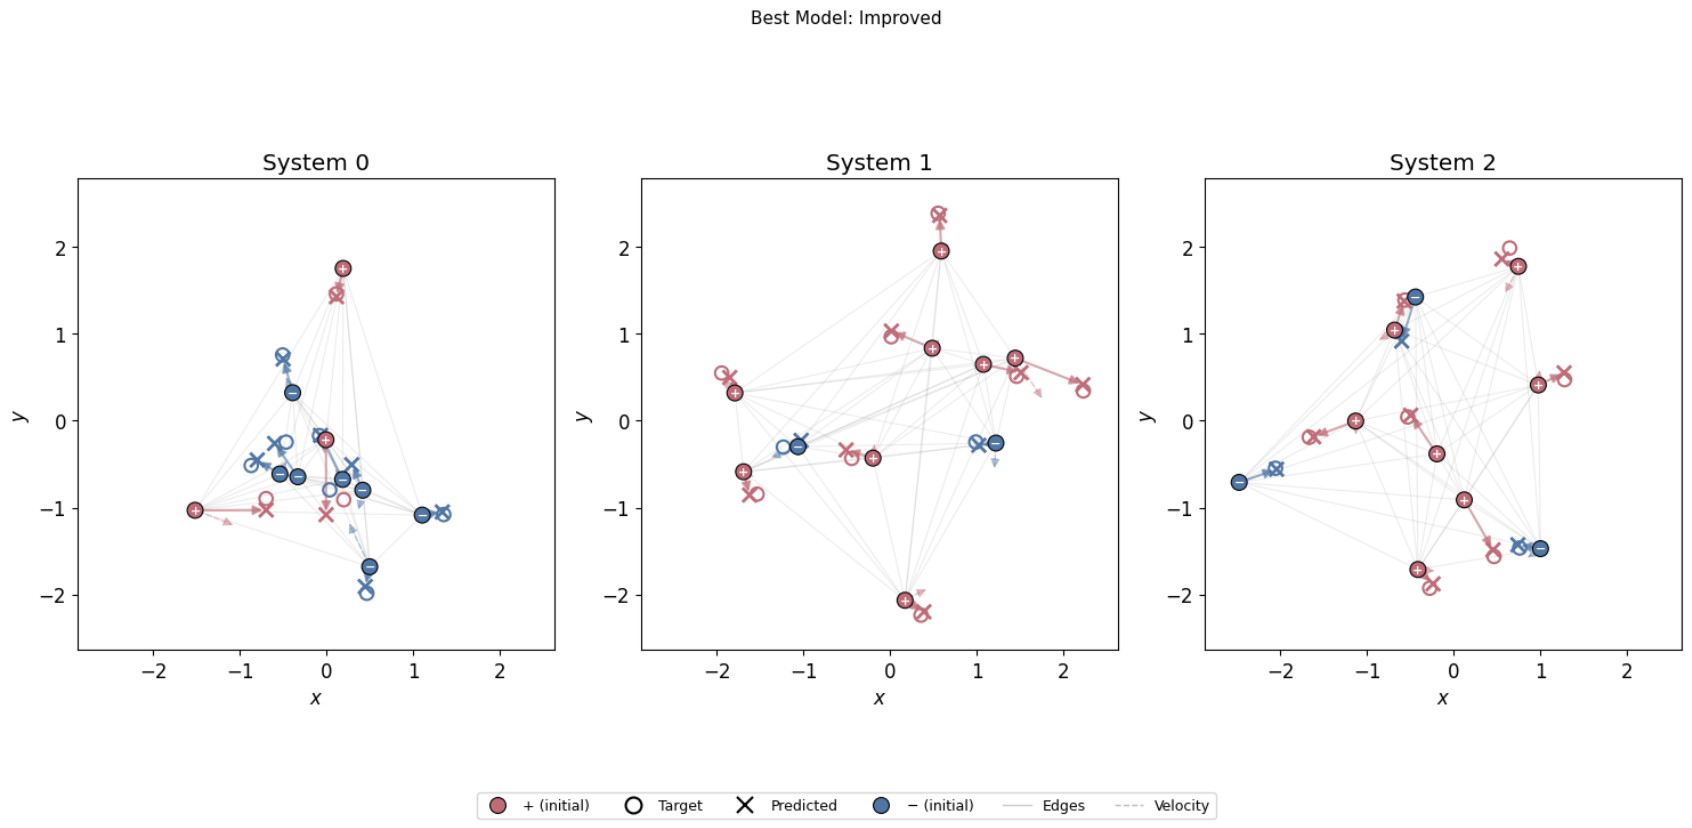
\includegraphics[width=\linewidth]{best_models.png}
    \caption{Predicted vs ground-truth trajectories for Improved Attention.}
  \end{minipage}\hfill
  \begin{minipage}{0.49\textwidth}
    \centering
    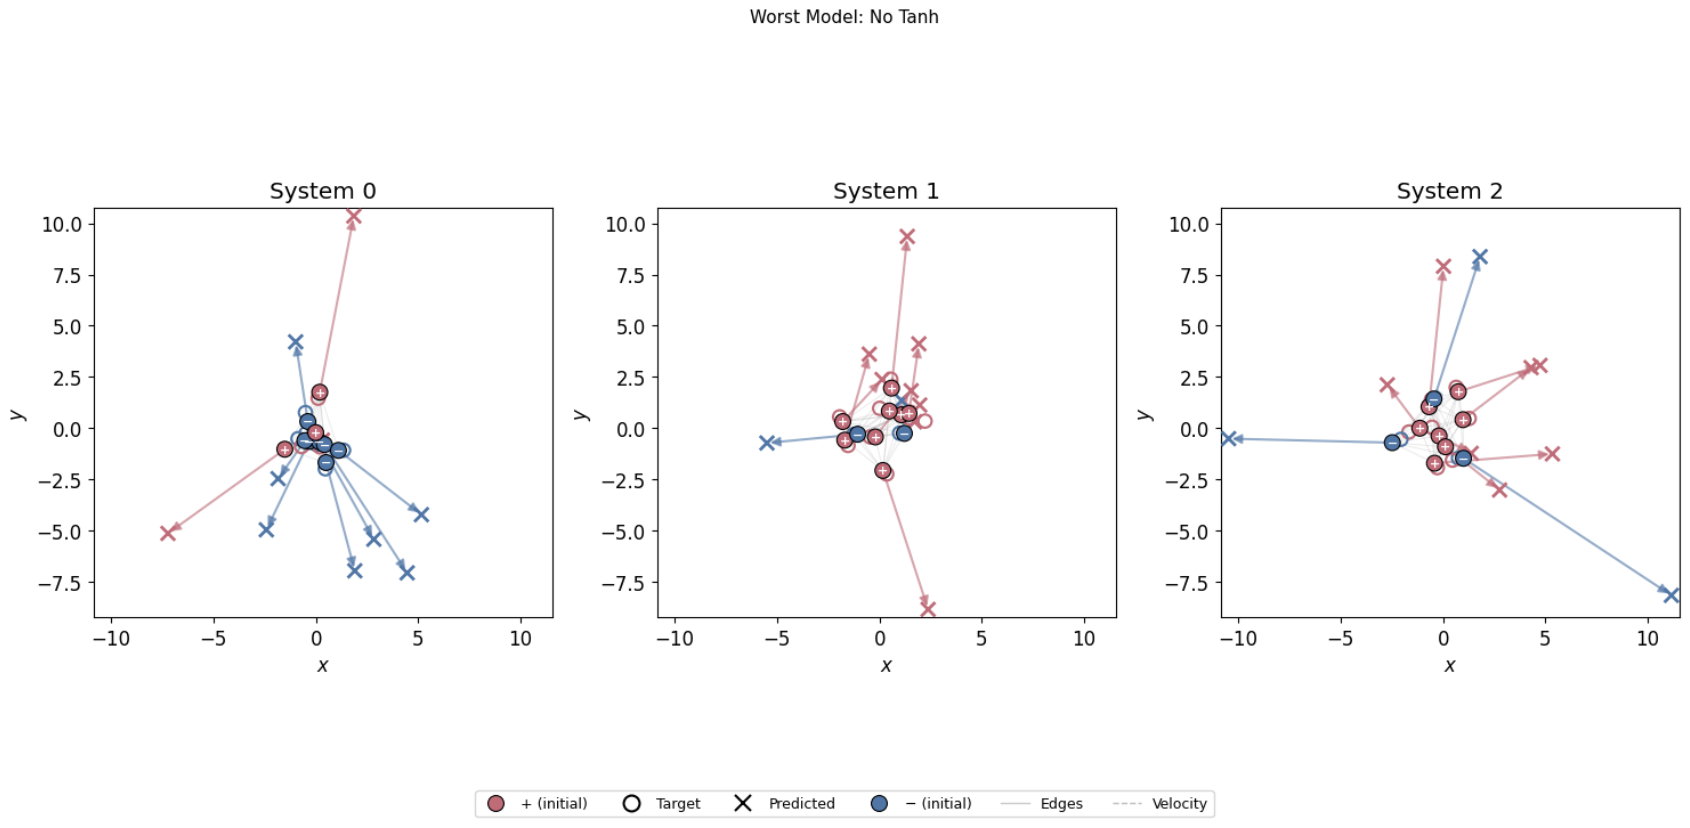
\includegraphics[width=\linewidth]{worst_models.png}
    \caption{Predicted vs ground-truth trajectories for No Tanh (divergent).}
  \end{minipage}
  \vspace{-0.3cm}
\end{figure}

\section{Discussion}

Comparing validations across the tested models reveals a clear categorization of EGNN components. Some drive absolute performance constraints while others are useful but secondary optimization tricks. 

\textbf{The cost of breaking equivariance.} Forcing the graph to rely on absolute coordinates in \texttt{egnn\_no\_equivariance.py} degrades model performance. Because physical interaction depends exclusively on relative vector topologies an EGNN must otherwise aggressively memorize specific training sub-spaces. This makes generalization to rotated validation examples effectively impossible. Even though its validation MSE is not the highest its Equivariance Error jumps by four orders of magnitude ($1.17 \times 10^{-2}$). As verified by this metric its predictions drift significantly and inconsistently under spatial rotation.

\textbf{Information sparsity without distance.} The \texttt{egnn\_no\_distance.py} ablation (0.1068 MSE) confirms that relying purely on charge features creates an impoverished representation. Coulomb Law dictates that force diminishes with the inverse square of distance. Without explicit geometric distances injected into the scalar messages the graph relies solely on implicit relative coordinate updates and severely oversimplifies predicted trajectories.

\textbf{Structural stability and residual networks.} The \texttt{egnn\_no\_tanh.py} and \texttt{egnn\_no\_residual.py} models offer insights into graph deep learning optimization. Removing residual connections starves deep internal nodes of compounding memory and caps effective performance just below the baseline EGNN. However removing coordinate tanh bounding entirely breaks the model. As seen in the worst model trajectories without the squashing function to bound velocity shifts a single large edge message produces arbitrarily large position corrections. This creates a feedback loop that shoots particles across the simulation domain leading to an explosive MSE of 26.08.

\textbf{Incorporating Attention.} Finally the generated attention mechanism in \texttt{egnn\_improved.py} provides far greater dynamic range. Standard EGNNs uniformly pool edge vectors. By scaling localized neighbor updates the attention variant gives the graph the capability to focus on strong near-field repulsions instead of being overwhelmed by weak interactions occurring from further distant particles dropping the MSE to an impressive 0.0092.

\section{AI Collaboration}

I used a pipeline with Gemini 3 models for this project. During the design phase Gemini 3 Pro came up with architectural ideas for the improved EGNN. I gave it context about the geometry of the Coulomb interactions so the ideas would be practical. Then I used Gemini 3 Deep Think as a judge to pick the best ablation candidates. It found potential problems with breaking equivariance that I needed to fix.

For the implementation, Google AI IDE Antigravity with Gemini 3.1-High helped me write the code in Jupyter notebooks quickly. One specific failure happened when Gemini 3 Flash suggested a spatial rotation that was not mathematically orthogonal. I caught this error by checking the generated transformation matrix for the missing identity property. If I had just used the AI code the equivariance test would have been biased. I treated the AI as a critic and argued with its logic instead of just accepting it. This partnership kept the math solid while making development faster.

\end{document}
